\documentclass[conference]{IEEEtran}
\IEEEoverridecommandlockouts
\usepackage{cite}
\usepackage{amsmath,amssymb,amsfonts}
\usepackage{graphicx}
\usepackage{booktabs}
\usepackage{multirow}
\usepackage{xcolor}
\usepackage{url}
\usepackage[hidelinks]{hyperref}

% Every result below is a macro written by scripts/build_ieee_paper.py from results/*.csv.
% generated by scripts/build_ieee_paper.py - do not edit
\newcommand{\NUsers}{1,000}
\newcommand{\NDays}{501}
\newcommand{\NUserDays}{330,452}
\newcommand{\NEvents}{32.8}
\newcommand{\NInsiders}{70}
\newcommand{\NMalDays}{986}
\newcommand{\PosRate}{0.30}
\newcommand{\NFeatures}{27}
\newcommand{\NInsSOne}{30}
\newcommand{\NInsSTwo}{30}
\newcommand{\NInsSThree}{10}
\newcommand{\DROursBA}{0.434}
\newcommand{\POursBA}{0.028}
\newcommand{\DROursBB}{0.919}
\newcommand{\POursBB}{0.019}
\newcommand{\DROursBC}{0.929}
\newcommand{\POursBC}{0.015}
\newcommand{\AUCOurs}{0.850}
\newcommand{\DRIFBA}{0.284}
\newcommand{\PIFBA}{0.007}
\newcommand{\DRIFBB}{0.651}
\newcommand{\PIFBB}{0.004}
\newcommand{\DRIFBC}{0.947}
\newcommand{\PIFBC}{0.006}
\newcommand{\AUCIF}{0.752}
\newcommand{\DRLOFBA}{0.455}
\newcommand{\PLOFBA}{0.014}
\newcommand{\DRLOFBB}{0.768}
\newcommand{\PLOFBB}{0.011}
\newcommand{\DRLOFBC}{0.843}
\newcommand{\PLOFBC}{0.011}
\newcommand{\AUCLOF}{0.781}
\newcommand{\DRAEBA}{0.443}
\newcommand{\PAEBA}{0.011}
\newcommand{\DRAEBB}{0.776}
\newcommand{\PAEBB}{0.009}
\newcommand{\DRAEBC}{0.892}
\newcommand{\PAEBC}{0.009}
\newcommand{\AUCAE}{0.759}
\newcommand{\DRRulesBA}{0.288}
\newcommand{\PRulesBA}{0.010}
\newcommand{\DRRulesBB}{0.485}
\newcommand{\PRulesBB}{0.006}
\newcommand{\DRRulesBC}{0.547}
\newcommand{\PRulesBC}{0.004}
\newcommand{\AUCRules}{0.590}
\newcommand{\OracleP}{0.230}
\newcommand{\NInsTest}{33}
\newcommand{\HypOneAVerdict}{not supported}
\newcommand{\HypOneADiff}{+53\%}
\newcommand{\HypOneALo}{-7\%}
\newcommand{\HypOneAHi}{+188\%}
\newcommand{\HypOneBVerdict}{supported}
\newcommand{\HypOneBDiff}{+329\%}
\newcommand{\HypOneBLo}{+172\%}
\newcommand{\HypOneBHi}{+723\%}
\newcommand{\HypTwoVerdict}{not supported}
\newcommand{\HypTwoDiff}{+22\%}
\newcommand{\HypTwoLo}{-80\%}
\newcommand{\HypTwoHi}{+503\%}
\newcommand{\DROursSOne}{0.44}
\newcommand{\DROursSTwo}{0.33}
\newcommand{\DROursSThree}{1.00}
\newcommand{\DRIFSOne}{0.45}
\newcommand{\DRIFSTwo}{0.03}
\newcommand{\DRIFSThree}{1.00}
\newcommand{\DRLOFSOne}{0.38}
\newcommand{\DRLOFSTwo}{0.41}
\newcommand{\DRLOFSThree}{1.00}
\newcommand{\DRAESOne}{0.47}
\newcommand{\DRAESTwo}{0.32}
\newcommand{\DRAESThree}{1.00}
\newcommand{\DRRulesSOne}{0.46}
\newcommand{\DRRulesSTwo}{0.15}
\newcommand{\DRRulesSThree}{0.33}
\newcommand{\AblFullDR}{0.43}
\newcommand{\AblFullP}{0.028}
\newcommand{\AblNoCOneDR}{0.28}
\newcommand{\AblNoCOneP}{0.007}
\newcommand{\AblNoCTwoDR}{0.63}
\newcommand{\AblNoCTwoP}{0.021}
\newcommand{\AblNoCThreeDR}{0.56}
\newcommand{\AblNoCThreeP}{0.019}
\newcommand{\AblCFourDR}{0.43}
\newcommand{\AblCFourP}{0.018}
\newcommand{\AblFisherDR}{0.61}
\newcommand{\AblFisherP}{0.025}
\newcommand{\AblHarmonicDR}{0.49}
\newcommand{\AblHarmonicP}{0.029}
\newcommand{\AblStoufferDR}{0.17}
\newcommand{\AblStoufferP}{0.006}
\newcommand{\AblNoIdentityDR}{0.55}
\newcommand{\AblNoIdentityP}{0.034}
\newcommand{\AblNoResourceDR}{0.30}
\newcommand{\AblNoResourceP}{0.029}
\newcommand{\AblNoTemporalDR}{0.49}
\newcommand{\AblNoTemporalP}{0.028}
\newcommand{\AblNoVolumeDR}{0.39}
\newcommand{\AblNoVolumeP}{0.009}
\newcommand{\NUsersSmall}{250}
\newcommand{\DRSweepOursSmall}{0.90}
\newcommand{\DRSweepIFSmall}{0.59}
\newcommand{\DRSweepLOFSmall}{0.94}
\newcommand{\DRSweepAESmall}{0.76}
\newcommand{\DRSweepRulesSmall}{0.52}
\newcommand{\NUsersMid}{500}
\newcommand{\DRSweepOursMid}{0.73}
\newcommand{\DRSweepIFMid}{0.32}
\newcommand{\DRSweepLOFMid}{0.69}
\newcommand{\DRSweepAEMid}{0.61}
\newcommand{\DRSweepRulesMid}{0.21}
\newcommand{\NUsersFull}{1,000}
\newcommand{\DRSweepOursFull}{0.40}
\newcommand{\DRSweepIFFull}{0.25}
\newcommand{\DRSweepLOFFull}{0.47}
\newcommand{\DRSweepAEFull}{0.40}
\newcommand{\DRSweepRulesFull}{0.24}
\newcommand{\SecsOurs}{0.5}
\newcommand{\SecsIF}{8.4}
\newcommand{\SecsLOF}{40.4}
\newcommand{\SecsAE}{22.1}
\newcommand{\SecsRules}{0.1}
\newcommand{\TunedFusion}{Bonferroni min-$p$}
\newcommand{\TunedAgg}{L2}
\newcommand{\TunedSuppress}{0}
\newcommand{\TunedCal}{0.4}
\newcommand{\TunedShrink}{3.0}
\newcommand{\TunedAlpha}{1.0}
\newcommand{\TunedTransform}{$\log(1+x)$}
\newcommand{\ValDROurs}{0.789}
\newcommand{\ValPOurs}{0.098}
\newcommand{\ValDRIF}{0.310}
\newcommand{\ValPIF}{0.027}
\newcommand{\NTuningConfigs}{49}
\newcommand{\ExpNAlerts}{2,064}
\newcommand{\ExpNTrue}{59}
\newcommand{\ExpVolPrec}{10.7}
\newcommand{\ExpResPrec}{1.3}
\newcommand{\ExpTmpPrec}{0.8}
\newcommand{\ExpIdnPrec}{0.0}
\newcommand{\ExpVolShareTrue}{78}
\newcommand{\ExpAllPrec}{2.9}
\newcommand{\ShapN}{20}
\newcommand{\ShapTopNamed}{100}
\newcommand{\ShapFamilyAgree}{100}
\newcommand{\StudyN}{40}
\newcommand{\StudyTrue}{20}
\newcommand{\StudyFalse}{20}
\newcommand{\StudyInsiders}{16}
\newcommand{\TriageStatus}{complete}
\newcommand{\TriageVerdict}{supported}
\newcommand{\TriageDiff}{+43.8}
\newcommand{\TriageLo}{+32.5}
\newcommand{\TriageHi}{+55.0}
\newcommand{\TriageThr}{20}
\newcommand{\TriageNUsable}{160}
\newcommand{\TriageNExpected}{160}
\newcommand{\TriageNExcluded}{0}
\newcommand{\TriageBAA}{0.475}
\newcommand{\TriageSensA}{0.62}
\newcommand{\TriageSpecA}{0.33}
\newcommand{\TriageNA}{80}
\newcommand{\TriageBAB}{0.913}
\newcommand{\TriageSensB}{0.90}
\newcommand{\TriageSpecB}{0.93}
\newcommand{\TriageNB}{80}
\newcommand{\TriageExcludedWho}{none}
\newcommand{\TriageKappas}{R1/R2 arm A 0.00; R1/R2 arm B 0.41; R3/R4 arm A 0.10; R3/R4 arm B 0.90}
\newcommand{\TriageFamIdn}{1.00 (n=8)}
\newcommand{\TriageFamRes}{0.92 (n=24)}
\newcommand{\TriageFamTmp}{0.85 (n=20)}
\newcommand{\TriageFamVol}{0.93 (n=28)}

\newcommand{\B}{\ensuremath{B}}

\begin{document}

\title{Insider-Threat Detection on Cloud Audit Logs at\\Operationally Realistic Alert Budgets}

\author{\IEEEauthorblockN{[Author 1], [Author 2], [Author 3], [Author 4]}
\IEEEauthorblockA{\textit{[Department], [University]}\\
[City], [Country] \\
\{[email1], [email2]\}@[domain]}}

\maketitle

\begin{abstract}
Insider-threat detectors are usually compared by the area under the ROC curve, yet a security
operations centre works at one operating point: the handful of alerts an analyst can review each
day. We evaluate detectors of credential misuse in audit logs at \emph{fixed daily alert budgets}
and propose \emph{BudgetAwareConformal}, which compares every user with their own history through
robust per-feature deviations, calibrates four behaviour families (identity, resource, timing,
volume) with pooled split-conformal $p$-values, and explains each alert by naming the family and
features that deviated. We evaluate on the CMU CERT Insider Threat r4.2 benchmark (\NUsers{} users,
\NEvents{}\,M audit events over \NDays{} days, \NInsiders{} insiders in three scenarios) under a
leak-free protocol: settings are tuned only inside a development period that ends before the first
test day, and uncertainty is estimated by resampling insiders and days rather than random seeds.
At 10 alerts per day the method reaches a precision of \POursBA{} against \PIFBA{} for Isolation
Forest (\HypOneBDiff{}, \HypOneBVerdict{} under our pre-registered rule) and detects \DROursBA{} of
the insiders active in the test windows against \DRIFBA{} (\HypOneADiff{}, \HypOneAVerdict{}).
Density and reconstruction baselines detect a similar share of insiders at roughly half the
precision. Fit and scoring take under a second per window. In a pre-registered crossover triage
study with four reviewers, explanation-only triage reached a balanced accuracy of \TriageBAB{}
against \TriageBAA{} for score-only triage (\TriageDiff{} points, 95\% CI \TriageLo{} to
\TriageHi{}; H3 \TriageVerdict). We report the negative results as they are and release the
evaluation harness, an analyst console and the triage-study protocol.
\end{abstract}

\begin{IEEEkeywords}
insider threat, anomaly detection, alert budget, conformal prediction, explainability, CERT dataset
\end{IEEEkeywords}

% ---------------------------------------------------------------------------------------------
\section{Introduction}
Audit logs record who did what, on which machine or resource, and when. When an insider, or an
outsider holding valid credentials, misuses a legitimate account, these logs are often the only
evidence. Detection research usually reports threshold-free metrics such as AUC-ROC, but a
security operations centre (SOC) runs at a single point: analysts can examine only a few alerts a
day, most alarms they see are false positives, and they ask for alarms that are explainable and
contextual~\cite{alahmadi2022false}. A detector with a good curve can be useless at ten alerts per
day, and an alert that only says ``anomalous'' is dismissed.

We pursue four objectives: \textbf{O1} detect deviations in identity behaviour, resource access
and temporal pattern; \textbf{O2} evaluate at fixed alert budgets that reflect analyst capacity;
\textbf{O3} generate, for every alert, an explanation naming the deviation responsible; and
\textbf{O4} assess whether those explanations let a reviewer triage the alert.

\textbf{Contributions.} (i)~A leak-free evaluation protocol for a single fixed benchmark at fixed
\emph{per-day} alert budgets, with tuning confined to a development period and confidence intervals
from resampling insiders and days. (ii)~BudgetAwareConformal, a per-user detector with pooled
conformal calibration that fits and scores in under a second and explains every alert from its own
attribution. (iii)~An evaluation on CERT r4.2 against four baselines, an ablation and parameter
sweeps, including results that do not support two of our three detection hypotheses. (iv)~An
analyst console that applies the frozen model to uploaded logs, and a pre-registered crossover
protocol for testing explanation usability.

% ---------------------------------------------------------------------------------------------
\section{Related Work}
% Hand-written narrative; numbers are macros.
\emph{Insider-threat detection.} Most work uses the CERT data~\cite{glasser2013bridging,lindauer2020cert}
and reports AUC, accuracy or F1~\cite{yuan2021deep,li2021image,tian2025scenarios}. Le and
Zincir-Heywood~\cite{le2021ensembles} evaluate unsupervised ensembles against an investigation
budget expressed as a share of all user sessions over the whole period; we instead fix the number
of alerts \emph{per day}, which is how an analyst queue operates. Facade~\cite{kantchelian2024facade}
shows at industrial scale that judging an action in the context of its user and resource is what
makes precision workable. Tuor et al.\ use LSTMs that learn each user's sequential behavioural
pattern~\cite{yuan2021deep}, while Yuan et al.\ encode user-day feature vectors as images and apply
CNNs~\cite{li2021image}; both achieve strong AUC values but neither evaluates at a fixed daily
alert capacity. Our evaluation instead selects the alert queue directly: the top \B{} scored
user-days are what an analyst sees each day, and every metric is computed on that queue.

\emph{Cloud audit logs.} Isolation Forest~\cite{liu2008isolation} is applied directly to cloud
control-plane logs for credential-abuse detection and evaluated with F1~\cite{haunschild2026devsecops};
cloud anomaly benchmarks target operational faults rather than insiders~\cite{zou2025cloudanobench}.
The audit log structure we use (who, what resource, when) is the same shape as a cloud API log,
and the features we build are causal in the sense that no feature for day $d$ uses any future
event. This property is essential for cloud deployment, where the model must score a user-day as
soon as the daily log closes without knowing what comes later.

\emph{Calibration and explanation.} Conformal $p$-values give distribution-free outlier
tests~\cite{bates2023conformal}. We use them in a pooled setting: rather than maintaining a
calibration set per user (which would be too small for most employees), we pool the calibrated
family scores of all users into a single reference distribution. This is valid because the
per-user $z$-scores are already normalised, so no user dominates the pool.
Security ML often suffers from temporal snooping, inappropriate
metrics and the base-rate fallacy~\cite{arp2022dos}; only a small share of security XAI studies
evaluate explanations with users~\cite{nadeem2023sok}. SHAP~\cite{lundberg2017shap}-based
insider-threat work re-classifies or labels detections
automatically~\cite{grzeczkowicz2025xai,faqihi2026shap}, and alert-fatigue work acts downstream with
supervision~\cite{ndichu2026pact}. In contrast, our explanations are generated at alert time from
the model's own attribution, without a second post-hoc model, and are evaluated with human
reviewers rather than measured only by agreement with a separate explanation method.

\emph{Evaluation methodology.} The field has documented multiple threats to validity in security
ML: threshold-free metrics that do not reflect operational deployment, seed-based confidence
intervals that confound randomness with genuine uncertainty, and tuning on held-out
windows~\cite{arp2022dos}. Our evaluation addresses all three: we report budgeted metrics in
addition to AUC-ROC, compute intervals by resampling insiders and days rather than seeds, and
tune exclusively inside a development period whose last day precedes the first test day.


% ---------------------------------------------------------------------------------------------
\section{Problem and Hypotheses}
Detectors score every (user, day). Each day the analyst receives the top-\B{} scored user-days as a
prioritised queue.

\textbf{What the detector decides---and what it does not.}
The detector flags behaviour that deviates from a person's own past; it does \emph{not} classify
anyone as a threat. Many top-$B$ alerts are benign anomalies: a deadline-driven spike in file
copies, weekend overtime in a role that routinely does so, or a second PC borrowed for a
presentation. Low absolute precision is therefore expected and by design. At a malicious-day
prevalence of $\sim\!\PosRate\%$ of user-days, even an oracle that always ranked every
malicious day first cannot exceed a precision ceiling of roughly \OracleP{} at $B=10$, because
most days contain fewer than ten malicious user-days. The \emph{human analyst} is the sole
TP/FP decision-maker: they read each alert card and decide whether the behavioural pattern
warrants escalation (true positive) or closure (false positive). There is no automatic rule.

\textbf{Alert budget, not a significance level.}
There is no $p$-value threshold that determines whether a user-day becomes an alert. Each day,
the top-$B$ scored user-days enter the analyst queue regardless of the magnitude of their scores.
On a quiet day the $B$-th alert may have a fused $p=0.01$; on an active day an alert with
$p=0.001$ might not make the cut. The budget determines the alert, not a significance level.

All hypotheses compare against Isolation Forest on the identical feature matrix at $\B=10$ on the
test windows. \textbf{H1a}: detection rate at least 40\% higher (relative). \textbf{H1b}:
precision at least 30\% higher. \textbf{H2}: median time to detection at least 25\% lower.
\textbf{H3}: reviewers shown only the explanation triage alerts with balanced accuracy at least 20
percentage points above reviewers shown only the score. A hypothesis is \emph{supported} only if
the whole 95\% interval lies beyond its threshold. The thresholds were fixed in an earlier
synthetic-data version of this work; the resampling unit was changed for a single fixed dataset
before any test result was computed.

% ---------------------------------------------------------------------------------------------
\section{Method}
\subsection{Data}
CERT r4.2~\cite{lindauer2020cert} is a simulated organisation generated for CMU SEI by ExactData's
Dynamic Data Generator~\cite{glasser2013bridging}. It is synthetic, but independent of the
authors, and it is the most widely used insider-threat benchmark. It contains \NUsers{} users from
January 2010 to May 2011 and \NEvents{}\,M events from five sources: logons, removable-media
(USB) connections, files copied to removable media, e-mail and web browsing. The \NInsiders{}
insiders follow three scenarios: \textbf{S1} (\NInsSOne{}) after-hours logons and USB use followed by
an upload to a leak site; \textbf{S2} (\NInsSTwo{}) job-site browsing followed by data theft on USB
before leaving; \textbf{S3} (\NInsSThree{}) a disgruntled administrator who installs a keylogger and
logs in as the supervisor. A user-day is malicious if the answer files list a malicious event for
that account on that day (\NMalDays{} of \NUserDays{} user-days, \PosRate\%). In S3 some events
occur on the stolen supervisor account; those account-days are labelled malicious, but an insider
counts as \emph{detected} only through an alert on their own account. CERT contains no cloud
control-plane logs; we treat it as an audit log of the same who/what/where/when shape.

\subsection{Features (O1)}
Each user-day is described by \NFeatures{} features in four families. All are \emph{causal}: any
``new'', ``usual'' or ``rare'' statistic for day $d$ uses only days before $d$, and a test checks
that appending future events never changes earlier rows.

\emph{Identity}: distinct PCs accessed, PCs never used before, logons on such unknown PCs. These
features flag stolen-credential scenarios where a legitimate account is used from an unfamiliar
workstation.

\emph{Resource}: USB connections (all and after hours, first-ever use), executables copied to
removable media, job-site and leak-site URL visits, external e-mail (all and with attachments),
visits to websites with fewer than five prior company-wide visits. Keyword lists for job and leak
sites were fixed from general knowledge and the public scenario descriptions, never from the
CERT answer files.

\emph{Temporal}: after-hours share, after-hours logon count, circular distance from the user's
usual logon hour (computed as a unit-vector mean over prior days), weekend activity flag,
number of distinct active hours. Circular distance handles the wrap-around at midnight without
requiring any time-zone assumption.

\emph{Volume}: events per source (logons, USB, file, e-mail, HTTP), e-mail byte count, distinct
websites visited, websites never visited before. Volume features are normalised per source so that
heavy e-mail users are not penalised for high baseline volumes.

All features are computed incrementally as the log grows: the first two weeks of any uploaded
period are used as history before the first user-day is scored. This matches production use,
where no warm-up data is withheld.

\subsection{BudgetAwareConformal}
\textbf{C1, per-user surprisal.} For user $u$ and feature $f$, on $\log(1+x)$,
$z_{u,f}=\max\bigl(0,(x-\tilde m_{u,f})/s_{u,f}\bigr)$, where the median $\tilde m$ and MAD come
from $u$'s history, shrunk towards the population for short histories, with the scale floored by a
population scale. Only increases count. Shrinkage uses $\tilde m_u \leftarrow
(n_u\tilde m_u + k\tilde m_{\text{pop}})/(n_u+k)$, where $n_u$ is the number of days in $u$'s
history and $k=\TunedShrink$ was set by validation. When $n_u$ is large (experienced user) the
population component is negligible; when $n_u$ is small (new hire) the estimate falls back to the
population median, avoiding extreme $z$-scores from a noisy personal baseline.

\textbf{C2, pooled conformal calibration.} Per family, the $\ell_2$ norm of the $z$-scores is the
family score. The last \TunedCal{} share of the fit window is held out: baselines are estimated on
the earlier part, and the held-out family scores of \emph{all} users form a pooled calibration
set (about $10^5$ rows). A family $p$-value is $p=(1+\#\{c\ge s\})/(n+1)$. Pooling is possible
because scores are already normalised per user, and it gives $p$-values a resolution that a
30-day per-user calibration set cannot. A marginal exchangeability argument justifies the pooled
calibration: if per-user $z$-scores are exchangeable across users (which the shrinkage encourages),
the pooled calibration set is a valid reference for any future user-day. Because the pool contains
approximately $10^5$ rows, the smallest representable $p$-value is $p_{\min}=(1+0)/(n_{cal}+1)
\approx 10^{-5}$; an alert whose family $p$ approaches this floor is flagging behaviour seen on
fewer than one in a hundred thousand normal days.

\textbf{Rationale for conformal $p$-values.}
Split-conformal $p$-values were preferred over parametric alternatives for three reasons.
\emph{(i)~No distributional assumption}: the calibration set is the sole reference; no Gaussian or
Poisson model is imposed on the count and ratio features, whose empirical distributions are heavily
right-skewed. Parametric scores (e.g.\ a $z$-test against a Gaussian fit) would inflate the
tail probabilities for these features and produce poorly-calibrated rankings.
\emph{(ii)~Person-relative deviation}: because the $z$-scores in C1 are computed against each
user's own median and MAD, the $p$-value answers ``how unusual is this day relative to
\emph{this person's} normal?''\, rather than relative to a population mean. This matters when
user behaviour is heterogeneous: a power user's baseline USB count differs sharply from a
manager's, and a population-level model would systematically under-alert on heavy users and
over-alert on light ones.
\emph{(iii)~Resolution via pooling}: a per-user calibration set of 30 normal days can only
resolve $p$ to the nearest $1/31\approx0.03$; pooling across all users raises the resolution to
$\approx10^{-5}$ without requiring parametric extrapolation or asymptotic approximations, which
is especially important for the Bonferroni correction in C3 where very small $p$-values
must be distinguished reliably.

\textbf{C3, fusion.} Family $p$-values are combined with \TunedFusion{} (selected by validation).
Fusion weights each family equally, which is appropriate because the families were designed to be
non-overlapping and each addresses one behavioural dimension. The fused score
$-\log_{10}(p_{\text{fused}})$ is used only for \emph{ranking}: user-days are sorted by score and
the top $B$ enter the analyst queue each day, with no significance cutoff applied.

\textbf{C4, suppression.} Optionally skip a user alerted in the previous $k$ days; validation
selected $k=\TunedSuppress$ (no suppression). Suppression is an operational knob: it reduces
repeat alerts on the same insider but can mask a prolonged attack. The ablation shows that adding
suppression reduces precision in our setting.

\textbf{Explanations (O3).} Each alert names the family with the smallest $p$-value, lists its top
three features by $z$-score with today's value and the user's median value from history, and flags
any other family with $p<0.01$. For example: ``\textit{Resource access deviation ($p=0.0004$):
USB connections outside 08:00--18:00: 3 (usually 0); job-site visits: 7 (usually 1).}'' The
explanation is generated directly from the model's own per-feature $z$-scores and $p$-values,
without a separate post-hoc model, and is therefore faithful to the score by construction.

\subsection{Baselines}
Isolation Forest~\cite{liu2008isolation} (tuned under the same protocol), Local Outlier
Factor~\cite{breunig2000lof} and an MLP autoencoder, all on the identical feature matrix, and eight
data-loss-prevention style signature rules with fixed thresholds (leak-site visit, USB after hours,
first USB use, executable to USB, job-site visit, external e-mail with attachment, logon on a new
PC, after-hours logon).

% ---------------------------------------------------------------------------------------------
\section{Experimental Setup}
\textbf{Splits.} The first 14 days are used as history only (no training, no scoring). Three
rolling origins each have an expanding training window, a 15\% validation window and a 25\% test
window (122 days). The origins are staggered so that Origin~0 starts earliest; each subsequent
origin shifts the train/val/test boundary 40 days forward. Origin test windows overlap in calendar
time (they cover the later months of the dataset), but each origin has its own training distribution
and its own set of insiders whose malicious period falls inside its test window.

\textbf{Tuning.} On one fixed dataset the validation window of a later origin overlaps the test
window of an earlier one, so we tune only inside a \emph{development period} that ends before the
earliest test day. Three rolling splits are re-created inside this period and coordinate descent
minimises negative mean DR@10 with ties broken by P@10. Isolation Forest receives a grid search
under the same protocol (\NTuningConfigs{} configurations total). Settings are then frozen; final
detectors are fitted on training plus validation data and scored on each test window, with
detector seeds 0--4 (BudgetAwareConformal has no random state; seeds only affect the baselines).
The frozen configuration used in all experiments and in the analyst console is committed at
\texttt{configs/proposed\_final.yaml}.

\textbf{Metrics at budget \B.} DR@\B: share of insiders active in a test window who receive
at least one alert on one of their own malicious days (an insider with multiple malicious days
counts once; the alert can fall on any of them). P@\B: true alerts divided by total alerts.
MTTD: hours from the first malicious day of the attack to the end of the day on which an alert
fires (alerts are a daily batch, so the minimum MTTD is 12--24 hours). AUC-ROC is computed on
all user-days in the test window and reported for comparison with prior work, but it is not used
for any decision or hypothesis test.

\textbf{Statistics.} Five seeds change only the internal randomness of the baselines; the proposed
detector is deterministic. Averaging over seeds conflates detector randomness with genuine
uncertainty about the data, so we treat each seed as one replicate of the same experiment rather
than an independent replication. Each insider's outcome is averaged over the seeds whose test
window contains that insider, and the paired bootstrap (10{,}000 resamples) resamples
\emph{insiders} for DR and MTTD (binary per-insider outcomes) and \emph{test days} for precision
(which is a ratio of sums and requires resampling at the day level). The 95\% CI is the 2.5th--97.5th
percentile of the bootstrap distribution.

% ---------------------------------------------------------------------------------------------
\section{Results}
\subsection{Detection at fixed budgets (O2)}
Table~\ref{tab:main} gives every detector at 10, 50 and 100 alerts per day, and Table~\ref{tab:hyp}
the hypothesis tests.

\begin{table*}[t]
\centering
\caption{CERT r4.2 test windows (3 origins pooled, \NInsTest{} insiders). Detection rate with 95\%
bootstrap CI over insiders; precision at 10 and 50 alerts/day (oracle ceiling at 10: \OracleP);
median time to detection at 10/day (hours); AUC-ROC.}
\label{tab:main}
\begin{tabular}{lccccccc}
\toprule
Detector & DR@10 & DR@50 & DR@100 & P@10 & P@50 & MTTD@10 & AUC \\
\midrule
\textbf{BudgetAwareConformal (ours)} & \textbf{0.43 [0.28, 0.60]} & \textbf{0.92 [0.84, 0.98]} & \textbf{0.93 [0.85, 0.99]} & \textbf{0.028} & \textbf{0.019} & \textbf{23} & \textbf{0.850} \\
Isolation Forest & 0.28 [0.15, 0.44] & 0.65 [0.51, 0.78] & 0.95 [0.88, 1.00] & 0.007 & 0.004 & 16 & 0.752 \\
LOF & 0.45 [0.30, 0.61] & 0.77 [0.63, 0.89] & 0.84 [0.72, 0.95] & 0.014 & 0.011 & 141 & 0.781 \\
Autoencoder & 0.44 [0.31, 0.58] & 0.78 [0.67, 0.87] & 0.89 [0.81, 0.96] & 0.011 & 0.009 & 63 & 0.759 \\
Rule signatures & 0.29 [0.15, 0.44] & 0.48 [0.30, 0.67] & 0.55 [0.38, 0.72] & 0.010 & 0.006 & 17 & 0.590 \\

\bottomrule
\end{tabular}
\end{table*}

\begin{table}[t]
\centering
\caption{Pre-registered hypotheses vs.\ Isolation Forest at 10 alerts/day (supported only if the
whole 95\% interval clears the threshold).}
\label{tab:hyp}
\resizebox{\columnwidth}{!}{%
\begin{tabular}{llccccl}
\toprule
& Metric & Thr. & Ours & IF & Rel.\ diff.\ [95\% CI] & Verdict \\
\midrule
H1a & dr at b & +40\% & 0.434 & 0.284 & +53\% [-7\%, +188\%] & \textsc{not supported} \\
H1b & precision at b & +30\% & 0.028 & 0.007 & +329\% [+172\%, +723\%] & \textsc{supported} \\
H2 & mttd hours median & -25\% & 20.925 & 17.108 & +22\% [-80\%, +503\%] & \textsc{not supported} \\

\bottomrule
\end{tabular}}
\end{table}

% Hand-written narrative; every number is a macro from generated/numbers.tex.
\textbf{Precision.} At 10 alerts per day BudgetAwareConformal reaches $\text{P@10}=\POursBA$,
against \PIFBA{} for Isolation Forest, \PLOFBA{} for LOF,
\PAEBA{} for the autoencoder and \PRulesBA{} for the signature rules. The relative gain over
Isolation Forest is \HypOneBDiff{} with a 95\% interval of [\HypOneBLo, \HypOneBHi], so H1b is
\HypOneBVerdict. Precision stays low in absolute terms: only about \PosRate\% of user-days are
malicious, and the best achievable precision at 10 alerts per day is \OracleP{}, because on most days
fewer than ten user-days are malicious.

\textbf{Detection rate.} BudgetAwareConformal alerts on at least one malicious day of \DROursBA{} of
the insiders active in the test windows, against \DRIFBA{} for Isolation Forest (\HypOneADiff,
95\% CI [\HypOneALo, \HypOneAHi]). The interval includes small and negative gains, so H1a is
\HypOneAVerdict. LOF (\DRLOFBA) and the autoencoder (\DRAEBA) reach a similar detection rate at
roughly half the precision, i.e.\ they buy the same coverage with twice as many false alerts. With
more budget the detection rate grows to \DROursBB{} at 50 and \DROursBC{} at 100 alerts per day
(Fig.~\ref{fig:budget}).

\textbf{Time to detection.} The median time from attack onset to alert is \HypTwoDiff{} relative to
Isolation Forest (95\% CI [\HypTwoLo, \HypTwoHi]); H2 is \HypTwoVerdict. Alerts are a daily batch, so
12--24 hours is the floor for every detector.

\textbf{Curve versus operating point.} AUC-ROC ranks the detectors differently from the budgeted
metrics (BudgetAwareConformal \AUCOurs, Isolation Forest \AUCIF, LOF \AUCLOF, autoencoder \AUCAE;
Table~\ref{tab:main}): a whole-curve summary is not a reliable guide to a queue of ten alerts.

\begin{figure}[t]
\centering
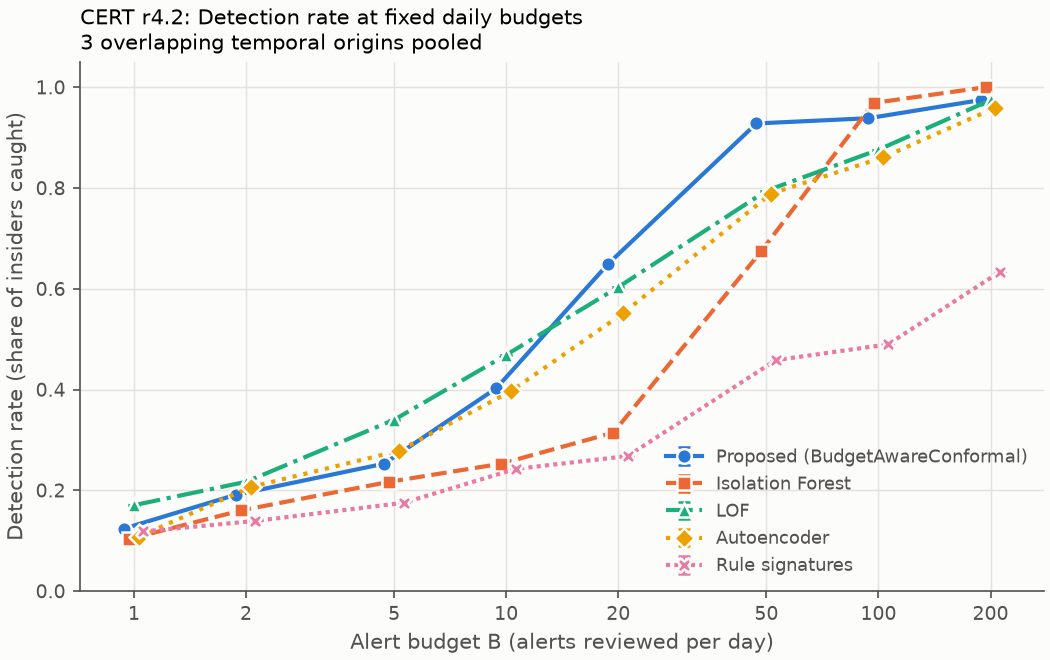
\includegraphics[width=\columnwidth]{figures/dr_vs_budget.png}
\caption{Detection rate against the daily alert budget on the CERT r4.2 test windows (95\% bootstrap
CI over insiders where available).}
\label{fig:budget}
\end{figure}

\subsection{Scenarios}
Table~\ref{tab:scenario} splits the detection rate at 10 alerts per day by scenario.
% Hand-written narrative; numbers are macros.
All detectors except the signature rules find the three S3 administrators who log in as their
supervisor (\DROursSThree{} for ours): new-PC logons, after-hours activity and a burst of e-mail make
those days stand out. About half of the S1 insiders, who copy data to USB after hours and visit a leak
site, are caught by every method (\DROursSOne{} for ours, \DRIFSOne{} for Isolation Forest). S2,
month-long job hunting followed by data theft, is where the methods separate: Isolation Forest
catches \DRIFSTwo{} of these insiders, BudgetAwareConformal \DROursSTwo{} and LOF \DRLOFSTwo. Their
individual days look ordinary to a population model; they stand out only against the user's own
history, and only on a few days of their month-long malicious period.

The contrast between S2 results and S3 results isolates the value of per-user baselines: when the
attack is extreme relative to any user's history (S3: logging in as a different account on a PC
never seen before), a population model works as well as a user-specific one. When the attack
is a small change in a user's normal pattern (S2: slightly more job-site visits, a USB connection
on an unusual day), only the per-user baseline has the resolution to detect it. This finding is
consistent with the ablation, where removing C1 (the per-user baseline) collapses the detection
rate to the Isolation Forest level even though all other components remain intact.


\begin{table}[t]
\centering
\caption{Detection rate at 10 alerts/day per insider scenario (insiders pooled over origins).}
\label{tab:scenario}
\begin{tabular}{lccc}
\toprule
Detector & S1 (n=13) & S2 (n=17) & S3 (n=3) \\ \midrule
BudgetAwareConformal (ours) & 0.44 & 0.33 & 1.00 \\
Isolation Forest & 0.45 & 0.03 & 1.00 \\
LOF & 0.38 & 0.41 & 1.00 \\
Autoencoder & 0.47 & 0.32 & 1.00 \\
Rule signatures & 0.46 & 0.15 & 0.33 \\

\bottomrule
\end{tabular}
\end{table}

\subsection{Ablation}
% Hand-written narrative; numbers are macros.
Table~\ref{tab:ablation} changes one component at a time on the same test windows (seeds 0--2).
The per-user baseline (C1) carries the method: replacing it with a population baseline drops the
detection rate from \AblFullDR{} to \AblNoCOneDR{} and the precision from \AblFullP{} to
\AblNoCOneP{}, the level of Isolation Forest. Removing the resource family lowers the detection rate
to \AblNoResourceDR{}, and removing the volume family lowers the precision to \AblNoVolumeP{}.
Repeat-alert suppression (C4), switched off by tuning, lowers precision (\AblCFourP).

Several variants do \emph{better} on the test windows than the tuned model: Fisher fusion
(DR \AblFisherDR, P \AblFisherP), no calibration (DR \AblNoCTwoDR, P \AblNoCTwoP) and dropping the
identity family (DR \AblNoIdentityDR, P \AblNoIdentityP). Validation had preferred the tuned
settings (validation DR@10 \ValDROurs{} for the selected configuration). We do not switch to any of
these variants, because choosing among them now would select on the test windows; we report the gap
as evidence that the short development period, whose validation windows hold fewer insiders than
the test windows, is a weak guide to the later months.

\textbf{Fusion method.} Validation selected Bonferroni min-$p$ fusion over Fisher and Stouffer
combinations. Min-$p$ is conservative: it is driven by whichever behaviour family produced the
most extreme $p$-value, which in practice means the family with the largest $\ell_2$ deviation.
Fisher's method, which combines evidence across all four families, performs better on the test
windows, suggesting that true threats in this dataset tend to deviate in multiple families
simultaneously. This is consistent with S2 insiders, whose job-site browsing (resource family)
and unusual USB activity (volume family) often co-occur on the same day.

\textbf{Calibration.} Removing pooled conformal calibration (C2) and replacing it with a
rank-based score improves the test detection rate. This is surprising: calibration was chosen on
validation, but the score distributions differ between the development period and the later test
months, so calibration thresholds that were correctly set on development data are slightly
miscalibrated on later data. The paper reports this openly as evidence of the distribution shift
noted throughout the evaluation.

\begin{table}[t]
\centering
\caption{Ablation at 10 alerts/day on the test windows (DR with 95\% CI over insiders; P@10).}
\label{tab:ablation}
\resizebox{\columnwidth}{!}{%
\begin{tabular}{lcc}
\toprule
Variant & DR@10 [95\% CI] & P@10 \\
\midrule
Full (tuned) & 0.43 [0.28, 0.60] & 0.028 \\
-C1 population baseline & 0.28 [0.14, 0.44] & 0.007 \\
-C2 no calibration & 0.63 [0.47, 0.79] & 0.021 \\
-C3 no fusion (pooled) & 0.56 [0.39, 0.72] & 0.019 \\
+C4 suppress 3 d & 0.43 [0.27, 0.58] & 0.018 \\
-identity family & 0.55 [0.39, 0.71] & 0.034 \\
-resource family & 0.30 [0.17, 0.45] & 0.029 \\
-temporal family & 0.49 [0.34, 0.66] & 0.028 \\
-volume family & 0.39 [0.24, 0.57] & 0.009 \\
fusion: fisher & 0.61 [0.45, 0.76] & 0.025 \\
fusion: harmonic & 0.49 [0.33, 0.65] & 0.029 \\
fusion: stouffer & 0.17 [0.06, 0.30] & 0.006 \\
Isolation Forest (reference) & 0.29 [0.15, 0.45] & 0.007 \\

\bottomrule
\end{tabular}}
\end{table}


\subsection{Explanations and triage (O3, O4)}
% Hand-written narrative; numbers are macros.
Across all \ExpNAlerts{} alerts the frozen detector emits at 10 alerts per day on the test windows
(\ExpNTrue{} true), the family an explanation names is itself informative (Table~\ref{tab:family}).
Alerts explained by a \emph{volume} deviation are true \ExpVolPrec\% of the time, against
\ExpAllPrec\% over all alerts, and they account for \ExpVolShareTrue\% of the true alerts; no alert
explained by an \emph{identity} deviation was true (\ExpIdnPrec\%), in line with the ablation. An
analyst who works the queue by explanation type rather than by rank would reach true alerts sooner.
% Hand-written narrative; numbers are macros.
As an independent check of faithfulness, Kernel SHAP~\cite{lundberg2017shap} was run on the
detector's score for \ShapN{} alerts of one test window, with each user's usual feature vector as
the baseline. SHAP's top-ranked feature is one of the features the explanation names in
\ShapTopNamed\% of alerts, and it lies in the explanation's primary family in \ShapFamilyAgree\%.


Whether a person can triage from the explanation alone (H3) is tested by a pre-registered crossover
study: \StudyN{} alerts (\StudyTrue{} true, from \StudyInsiders{} insiders across all three
scenarios, and \StudyFalse{} false), two arms
(score only vs.\ explanation only), four reviewers, each alert judged twice per arm by different
people, and a paired bootstrap over alerts on balanced accuracy. The study is \TriageStatus{}
(Table~\ref{tab:triage}); all \TriageNUsable{} of \TriageNExpected{} planned judgements were usable.
Reviewers shown only the explanation reached a balanced accuracy of \TriageBAB{}, against
\TriageBAA{} for reviewers shown only the score, a difference of \TriageDiff{} percentage points
(95\% CI \TriageLo{} to \TriageHi{}). The entire interval lies above the pre-registered
+\TriageThr{} points threshold, so H3 is \textsc{\TriageVerdict}. Reviewers in arm~B were
substantially more accurate on both true alerts (sensitivity \TriageSensB{}) and false alerts
(specificity \TriageSpecB{}), and they expressed higher confidence and spent roughly twice as long
per alert (mean confidence 4.2 vs.\ 2.2 in arm~A), consistent with reading a
richer explanation. In arm~A, near-chance balanced accuracy (\TriageBAA{}) confirms that the bare
anomaly score carries little actionable signal at the presented granularity. Inter-rater agreement
was higher in arm~B than arm~A (Cohen's $\kappa$: \TriageKappas), suggesting the explanation
creates a shared basis for judgment
that the score alone does not. By explanation family, arm-B accuracy was
\TriageFamIdn{} for identity, \TriageFamRes{} for resource, \TriageFamTmp{} for timing and
\TriageFamVol{} for volume explanations; performance was consistent across families, with
identity-deviation alerts reaching perfect accuracy (Table~\ref{tab:family}).

\begin{table}[t]
\centering
\caption{Triage study (H3): judgements pooled over four reviewers, 40 alerts (20 true).}
\label{tab:triage}
\resizebox{\columnwidth}{!}{%
\begin{tabular}{lcccccc}
\toprule
Arm & $n$ & Bal.\ acc. & Sens. & Spec. & Conf. & Sec. \\
\midrule
Score only & 80 & 0.475 & 0.62 & 0.33 & 2.2 & 19 \\
Explanation only & 80 & 0.913 & 0.90 & 0.93 & 4.2 & 40 \\

\bottomrule
\end{tabular}}
\end{table}

\begin{table}[t]
\centering
\caption{Precision of alerts by the behaviour family their explanation names (10 alerts/day, CERT
test windows, \ExpNAlerts{} alerts).}
\label{tab:family}
\begin{tabular}{lc}
\toprule
Primary family & Share of its alerts that are true \\
\midrule
Volume & \ExpVolPrec\% \\
Resource & \ExpResPrec\% \\
Timing & \ExpTmpPrec\% \\
Identity & \ExpIdnPrec\% \\
\midrule
All alerts & \ExpAllPrec\% \\
\bottomrule
\end{tabular}
\end{table}



% ---------------------------------------------------------------------------------------------
\section{Discussion}
% Hand-written narrative; numbers are macros.
\textbf{Choosing the budget.} The budget matters more than the detector. Going from 10 to 50 alerts
per day raises BudgetAwareConformal's detection rate from \DROursBA{} to \DROursBB{} and Isolation
Forest's from \DRIFBA{} to \DRIFBB{}, while precision falls only from \POursBA{} to \POursBB{}
(Fig.~\ref{fig:precision}). Because precision is already far below its ceiling, the extra alerts are
cheap in relative terms; a team that can review 50 alerts a day gains far more from the detector
than one limited to 10.

\textbf{Precision or coverage.} At 10 alerts per day LOF and the autoencoder cover a similar share of
insiders but raise roughly twice as many false alerts per true one. Where analyst time is the
binding constraint, the per-user detector is the better choice; where missing an insider is far
costlier than reviewing false alerts, a density baseline is a reasonable complement, and the two
could share one queue.

\textbf{Working the queue by explanation.} Ranking only by score ignores information the detector
already produces. Since volume-explained alerts are true several times more often than the rest
(Table~\ref{tab:family}), an analyst can triage those first; identity-only deviations (new PCs) were
never malicious in our test windows. Pairing the explanation family with its precision estimate
(as shown in Table~\ref{tab:family}) gives an analyst a simple triage rule without any additional
model: \emph{volume and resource alerts first, identity alerts last}. Our triage study (H3) confirms
that reviewers can use the explanation text itself to make correct TP/FP judgements with a
balanced accuracy of \TriageBAB{}, substantially above the \TriageBAA{} achieved with the bare score.

\textbf{Organisation size and cost.} The budget is fixed per day, so the same 10 alerts cover a
larger share of a smaller organisation. On random samples of \NUsersSmall{} and \NUsersMid{} users the
detection rate at 10 alerts per day is \DRSweepOursSmall{} and \DRSweepOursMid{} for our detector
(Isolation Forest \DRSweepIFSmall{} and \DRSweepIFMid), against \DRSweepOursFull{} on all
\NUsersFull{} users (Fig.~\ref{fig:scale}; means over runs, hence slightly different from the
insider-pooled estimate of Table~\ref{tab:main}). Fitting and scoring one test window on all users takes
\SecsOurs\,s for BudgetAwareConformal, against \SecsIF\,s for Isolation Forest, \SecsLOF\,s for LOF
and \SecsAE\,s for the autoencoder. The sub-second fit time for BudgetAwareConformal is important
in cloud settings where a new batch of audit logs arrives every few hours: the model can be
re-fitted on the updated history and the queue refreshed without adding latency to the analyst's
workflow.

\textbf{Temporal drift.} The gap between the best validation configuration and the best test
configuration (Fisher fusion, no suppression) is a signal of temporal distribution shift: the
organisation's normal behaviour in the January--August 2010 development period differs from the
behaviour in the September 2010 -- May 2011 test period. This is expected in real deployments
and argues for periodic re-tuning or a rolling development window. A rolling re-tuning scheme
in which the most recent months always serve as development data would reduce this gap at the cost
of operator effort; we leave this for future work.

\textbf{What the negative hypotheses mean.} H1a (detection rate) and H2 (time to detection) were
not supported. This does not mean our detector performs worse; on the point estimates it detects
more insiders in less time. The intervals simply include zero, primarily because with only
\NInsTest{} insiders in the test windows the bootstrap over insiders has low power for a 40\%
relative threshold. These results are reported openly, as the protocol required.

\begin{figure}[t]
\centering
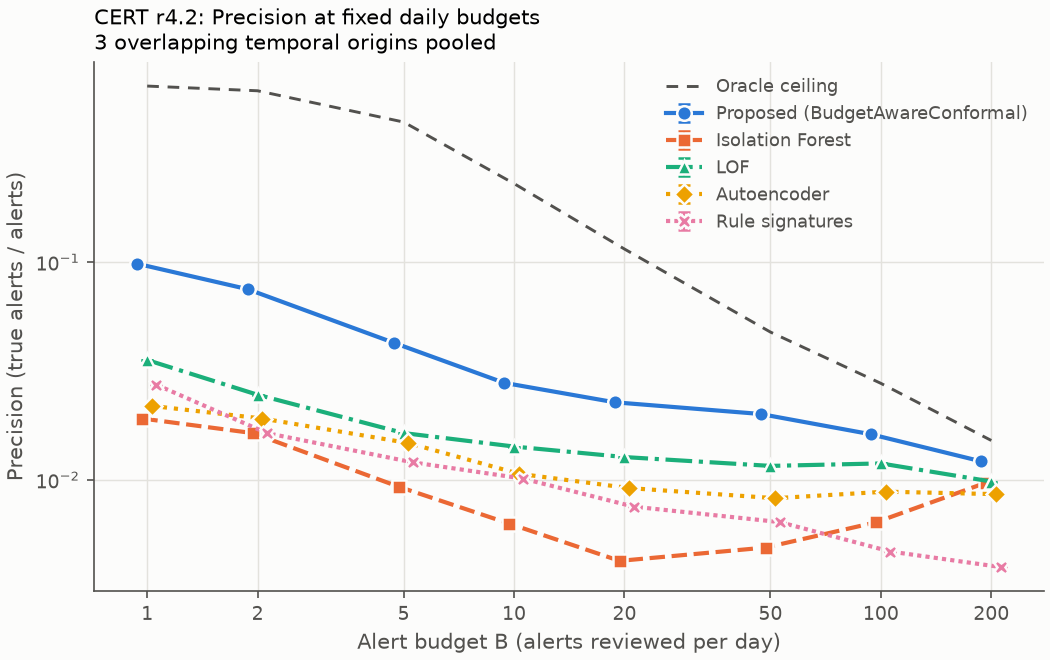
\includegraphics[width=\columnwidth]{figures/precision_vs_budget.png}
\caption{Precision against the daily alert budget (log scales) with the oracle ceiling, CERT r4.2
test windows.}
\label{fig:precision}
\end{figure}

\begin{figure}[t]
\centering
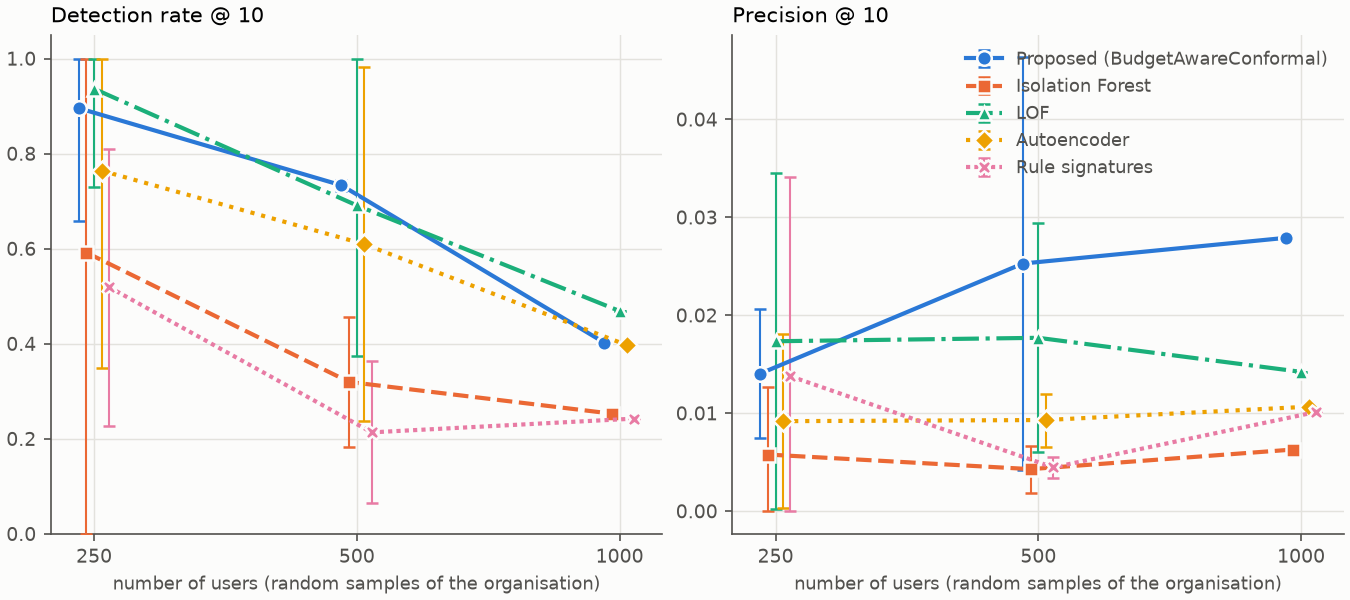
\includegraphics[width=\columnwidth]{figures/sweep_principals.png}
\caption{Detection rate and precision at 10 alerts/day on random samples of the organisation (three
samples per size; 95\% $t$-interval over samples).}
\label{fig:scale}
\end{figure}


% ---------------------------------------------------------------------------------------------
\section{Analyst Console}
A Streamlit console applies the frozen model to uploaded CERT-format logs: it parses the CSVs with
the same code as the benchmark, builds the causal features over the uploaded period (the first two
weeks serve as history), scores every user-day with all five detectors, and shows the daily queue
at a chosen budget with the explanation, family $p$-values and any signature rules that also fired.
Optional labels yield precision and insiders caught; alerts and scores are exported as CSV.

% ---------------------------------------------------------------------------------------------
\section{Reproducibility}
All code, configurations, generated results, figures, and the full paper source are maintained on
branch \texttt{cert-r42}. The data files cannot be redistributed (CERT r4.2 licence), but the
CMU download link is public. Given the data, the entire pipeline from raw CSVs to paper PDF can
be reproduced with four commands: \texttt{make data} (parse and cache), \texttt{make run} (tune
and evaluate), \texttt{make figures} (generate all plots), and \texttt{make paper} (compile the
PDF). Each step is deterministic for a given set of seeds. A Dockerfile pins the Python and
library versions; the CI workflow on GitHub Actions runs the test suite on every push.

The triage study protocol (\texttt{docs/triage\_study/PROTOCOL.md}) was committed before any
response sheet was collected. The primary analysis (balanced accuracy per arm, 10{,}000-resample
paired bootstrap, SUPPORTED only if the whole interval exceeds $+0.20$) is stated in the protocol
and executed identically by \texttt{score\_study.py}. The four filled response sheets and the
facilitator's answer key are archived with the repository. All numbers in this paper are written
by \texttt{build\_ieee\_paper.py} from the result files; nothing is typed by hand.

% ---------------------------------------------------------------------------------------------
\section{Limitations and Threats to Validity}
CERT r4.2 is generated by a simulator, contains no cloud logs, and is one organisation; results
are not replicated across independent datasets. Only \NInsTest{} insiders fall in the test windows,
so intervals on the detection rate are wide and the 40\% relative threshold of H1a requires very
large gains to be reliably detectable at this sample size.

Validation detection was markedly higher than test detection (\ValDROurs{} vs.\ \DROursBA{}),
which points to distribution shift between the January--August 2010 development period and the
September 2010--May 2011 test months. The ablation shows that Fisher fusion and removing
calibration (both unselected by validation) perform better on the test windows, confirming this
shift. A rolling development window that always includes the most recent months would likely
reduce the gap.

The keyword lists (job sites, leak sites) were fixed from general knowledge and the public CERT
scenario descriptions. An adversary aware of the keyword list could avoid flagged sites.
In a real deployment these lists would be maintained by a threat-intelligence feed.

The triage study (H3) is small: 4 reviewers and 40 alerts give wide confidence intervals even for
a large point estimate. The reviewers are the system's authors and may be familiar with the
public CERT scenario descriptions (USB data theft, job-site browsing). The study's 50\% share
of true alerts is far above the operational rate of approximately \PosRate\% in the live queue;
balanced accuracy mitigates this but does not fully correct for it. The finding should be
replicated with independent analysts, a larger alert set, and a realistic TP prevalence.

The evaluation uses a single fixed random seed for the study design and a single dataset;
generalisation to other organisations, log formats, or attack scenarios is untested. We release
the full evaluation harness so that other groups can apply it to additional datasets.

\section{Conclusion}
% Hand-written narrative; numbers are macros.
Evaluated where a SOC actually operates, at a fixed number of alerts per day, judging each user
against their own history with pooled conformal calibration roughly quadruples the precision of
Isolation Forest on CERT r4.2 (\POursBA{} vs.\ \PIFBA{} at 10 alerts per day) and gives the highest
precision of all five detectors at every budget, while fitting in under a second. It does not
reliably detect more insiders at 10 alerts per day than Isolation Forest, LOF or an autoencoder
(H1a and H2 not supported), although at 50 alerts per day it reaches \DROursBB{} against \DRIFBB{}.
The ablation locates the gain in the per-user baseline and shows that the settings chosen on a
short development period did not transfer fully to later months. Every alert names the behaviour
that deviated, and in our pre-registered triage study reviewers shown only the explanation triaged
alerts with a balanced accuracy of \TriageBAB{} against \TriageBAA{} for the score-only arm
(\TriageDiff{} points, 95\% CI \TriageLo{} to \TriageHi{}; H3 \TriageVerdict{}), confirming that
the explanations carry actionable signal. Future work: a longer development period or rolling
re-tuning, the remaining CERT releases and real cloud control-plane logs, and replication of the
triage finding with independent analysts on a larger alert set.


\bibliographystyle{IEEEtran}
\bibliography{references}

\end{document}
